\chapter{Hasil dan Pembahasan}

Bab ini akan membandingkan respon sistem dari skenario 1, skenario 2, dan skenario 3 ketika pasca gangguan. Fokus utama adalah analisis stabilitas sistem dengan memperhatikan osilasi elektromekanis, terkhususnya pada kecepatan dan sudut rotor.




\section{Perbandingan Skenario 1 dan Skenario 2}

Bagian ini akan menggambarkan efek dari penetrasi SPV pada stabilitas transien sistem tenaga listrik.



\subsection{Dampak ke Kecepatan Rotor Generator 1}

\begin{figure}[ht]
    \centering
    \begin{subfigure}[b]{0.49\linewidth}
        \centering
        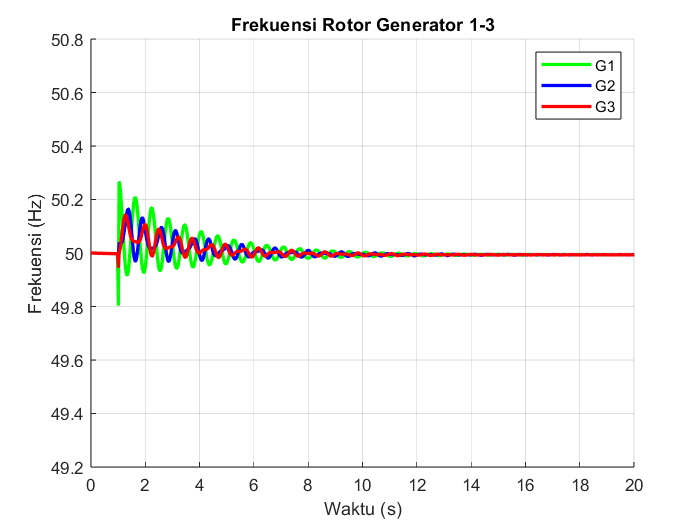
\includegraphics[width=\linewidth]{contents/chapter-4/frek-baseline-fault1.png}
        \caption{Skenario 1}
        \label{Fig:frek-baseline-fault1}
    \end{subfigure}
    \hfill
    \begin{subfigure}[b]{0.49\linewidth}
        \centering
        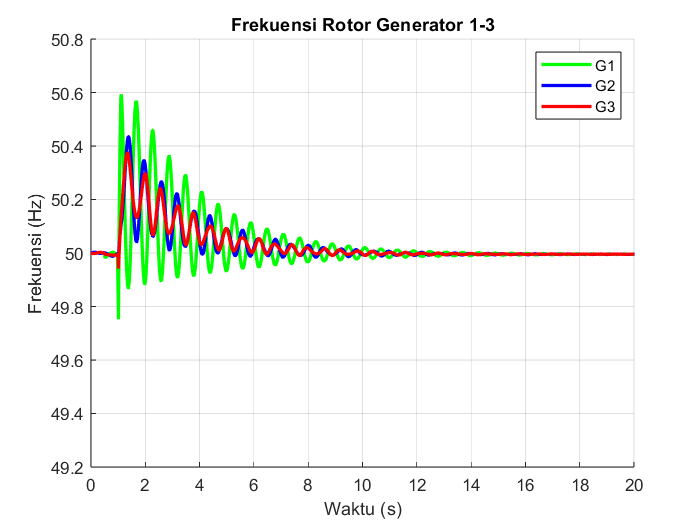
\includegraphics[width=\linewidth]{contents/chapter-4/frek-pv-fault1.png}
        \caption{Skenario 2}
        \label{Fig:frek-pv1-fault1}
    \end{subfigure}
    \caption{Plot Kecepatan Rotor, Gangguan di Bus 1.}
    \label{Fig:frek12-fault1}
\end{figure}

Dari Gambar \ref{Fig:frek12-fault1} terlihat \textit{overshoot} kecepatan rotor meningkat dari 1,06\% pada skenario 1 menjadi 2,89\% pada skenario 2. \textit{Undershoot} juga mengalami peningkatan dari 0,38\% menjadi 0,61\%. Demikian juga \textit{settling time} mengalami kenaikan dari 3,08 detik menjadi 5,54 detik. Sementara itu, \textit{steady state error} tidak mengalami perubahan signifikan, hanya berselisih $9,5 \times 10^{-5}$ p.u. antara kedua skenario.

\begin{figure}[ht]
    \centering
    \begin{subfigure}[b]{0.49\linewidth}
        \centering
        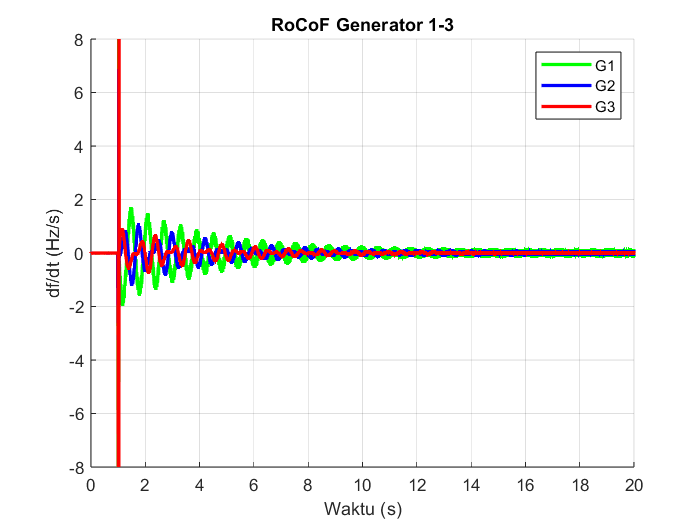
\includegraphics[width=\linewidth]{contents/chapter-4/rocof-baseline-fault1.png}
        \caption{Skenario 1}
        \label{Fig:rocof-baseline-fault1}
    \end{subfigure}
    \hfill
    \begin{subfigure}[b]{0.49\linewidth}
        \centering
        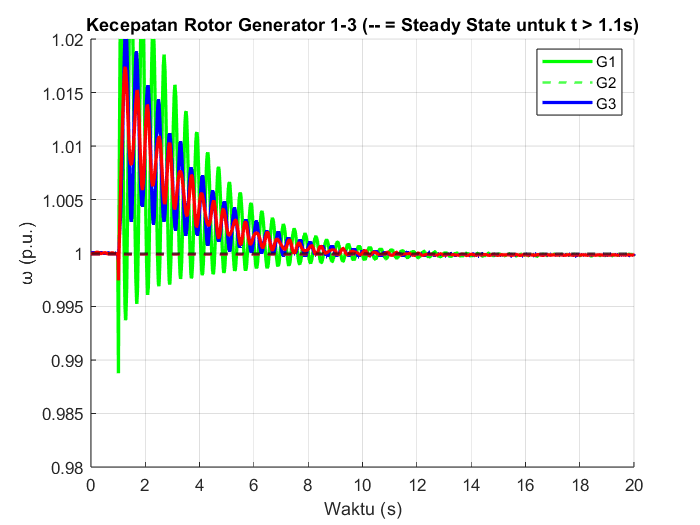
\includegraphics[width=\linewidth]{contents/chapter-4/rocof-pv-fault1.png}
        \caption{Skenario 2}
        \label{Fig:rocof-pv1-fault1}
    \end{subfigure}
    \caption{Plot \textit{RoCoF} dari Gambar \ref{Fig:frek12-fault1}, Gangguan di Bus 1.}
    \label{Fig:rocof12-fault1}
\end{figure}

Gambar \ref{Fig:rocof12-fault1} menunjukkan bahwa puncak \textit{RoCoF}, baik positif maupun negatif mengalami peningkatan cukup signifikan. Pada skenario 1, puncak \textit{RoCoF} mencapai 6,62 Hz/s dan -7,26 Hz/s. Sementara pada skenario 2, puncak \textit{RoCoF} menjadi 14,97 Hz/s dan -14,48 Hz/s.

\begin{figure}[ht]
    \centering
    \begin{subfigure}[b]{0.49\linewidth}
        \centering
        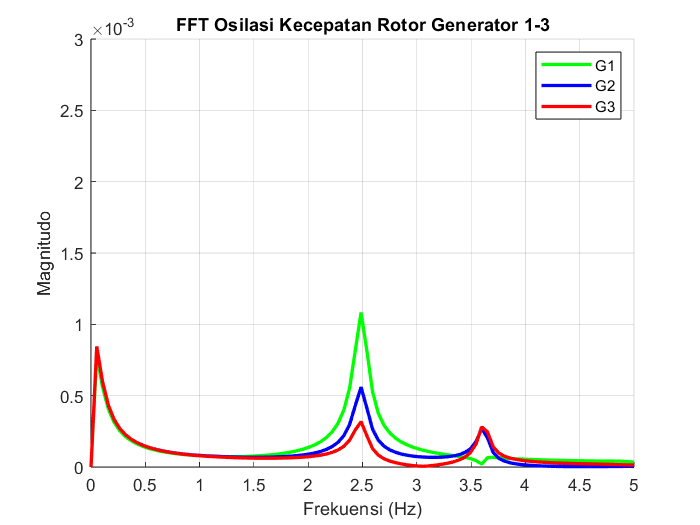
\includegraphics[width=\linewidth]{contents/chapter-4/fft-baseline-fault1.png}
        \caption{Skenario 1}
        \label{Fig:fft-baseline-fault1}
    \end{subfigure}
    \hfill
    \begin{subfigure}[b]{0.49\linewidth}
        \centering
        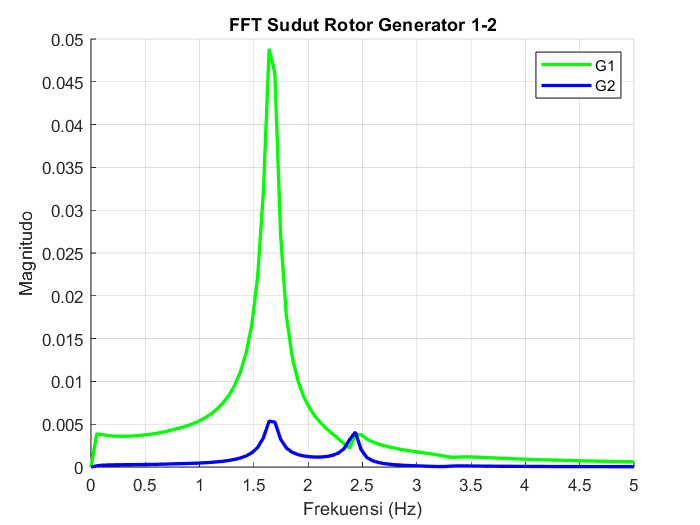
\includegraphics[width=\linewidth]{contents/chapter-4/fft-pv-fault1.png}
        \caption{Skenario 2}
        \label{Fig:fft-pv1-fault1}
    \end{subfigure}
    \caption{Plot \textit{FFT} Kecepatan Rotor dari Gambar \ref{Fig:frek12-fault1}, Gangguan di Bus 1.}
    \label{Fig:fft12-fault1}
\end{figure}

Hasil FFT dari plot kecepatan rotor ditunjukkan pada Gambar \ref{Fig:fft12-fault1}. Frekuensi kritis yang dominan pada kedua skenario sama persis di 2,5 Hz. Namun, amplitudonya pada skenario 2 meningkat secara signifikan dibandingkan dengan skenario 1.



\subsection{Dampak ke Sudut Rotor Generator 1}

\begin{figure}[ht]
    \centering
    \begin{subfigure}[b]{0.49\linewidth}
        \centering
        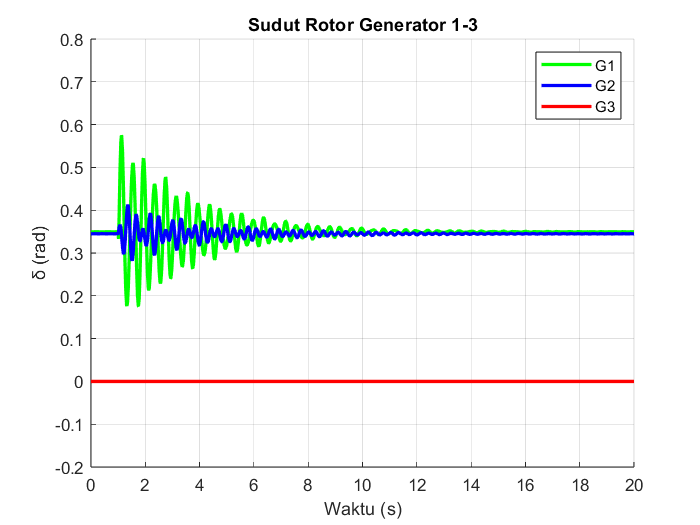
\includegraphics[width=\linewidth]{contents/chapter-4/ang-baseline-fault1.png}
        \caption{Skenario 1}
        \label{Fig:ang-baseline-fault1}
    \end{subfigure}
    \hfill
    \begin{subfigure}[b]{0.49\linewidth}
        \centering
        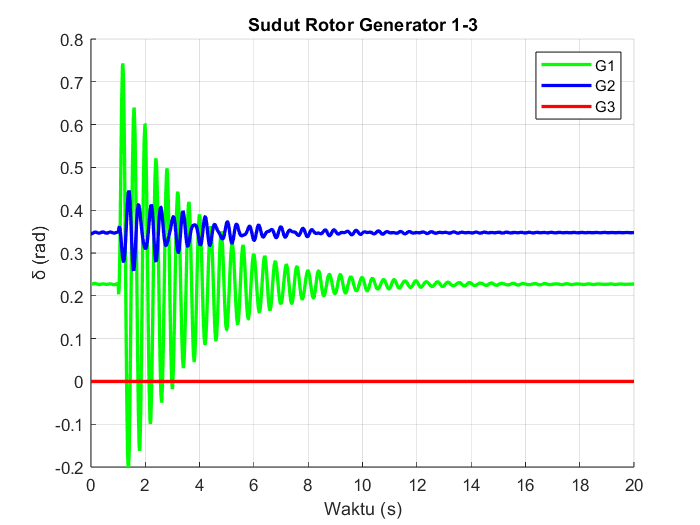
\includegraphics[width=\linewidth]{contents/chapter-4/ang-pv-fault1.png}
        \caption{Skenario 2}
        \label{Fig:ang-pv1-fault1}
    \end{subfigure}
    \caption{Plot Sudut Rotor, Gangguan di Bus 1.}
    \label{Fig:ang12-fault1}
\end{figure}

Sudut rotor pada Gambar \ref{Fig:ang12-fault1} menunjukkan pergeseran sudut rotor pada skenario 2 akibat penetrasi SPV. Deviasi maksimum sudut rotor meningkat dari 0.22 rad pada skenario 1 menjadi 0.52 rad pada skenario 2.



\subsection{Data Hasil Keseluruhan}




\section{Perbandingan Skenario 2 dan Skenario 3}



\subsection{Dampak ke Kecepatan Rotor}

\begin{figure}[ht]
    \centering
    \begin{subfigure}[b]{0.49\linewidth}
        \centering
        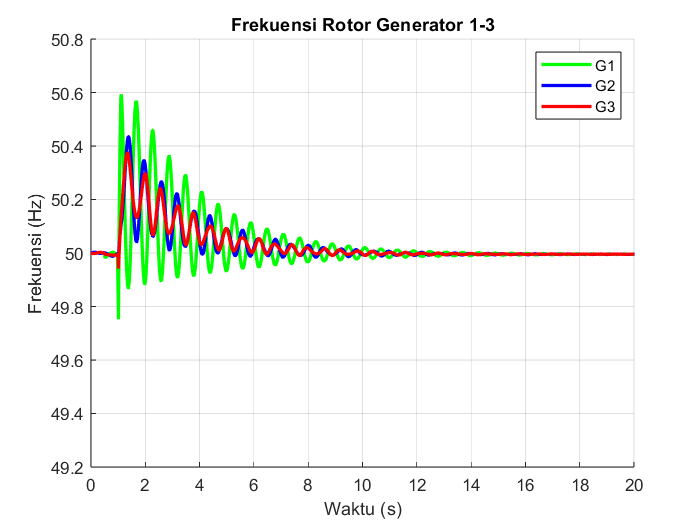
\includegraphics[width=\linewidth]{contents/chapter-4/frek-pv-fault1.png}
        \caption{Skenario 2}
        \label{Fig:frek-pv2-fault1}
    \end{subfigure}
    \hfill
    \begin{subfigure}[b]{0.49\linewidth}
        \centering
        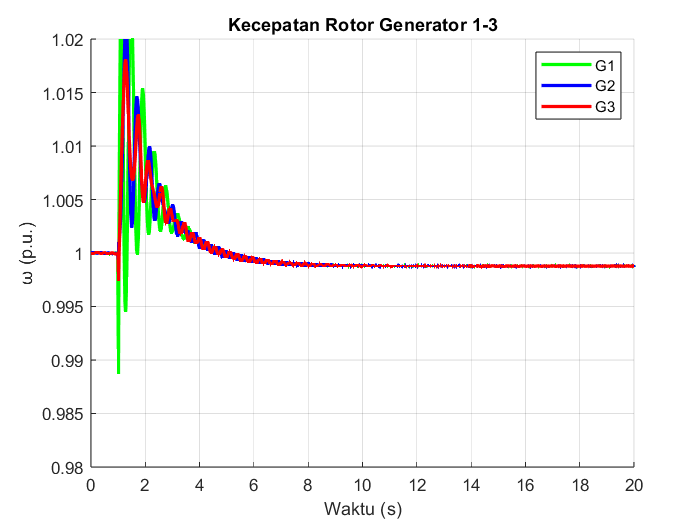
\includegraphics[width=\linewidth]{contents/chapter-4/frek-vi-fault1.png}
        \caption{Skenario 3}
        \label{Fig:frek-vi-fault1}
    \end{subfigure}
    \caption{Plot Kecepatan Rotor, Gangguan di Bus 1: (a) Skenario 2; (b) Skenario 3}
    \label{Fig:frek23-fault1}
\end{figure}

Pada \ref{Fig:frek-pv2-fault1} terlihat ... sementara pada \ref{Fig:frek-vi-fault1} terlihat bahwa ...

\begin{figure}[ht]
    \centering
    \begin{subfigure}[b]{0.49\linewidth}
        \centering
        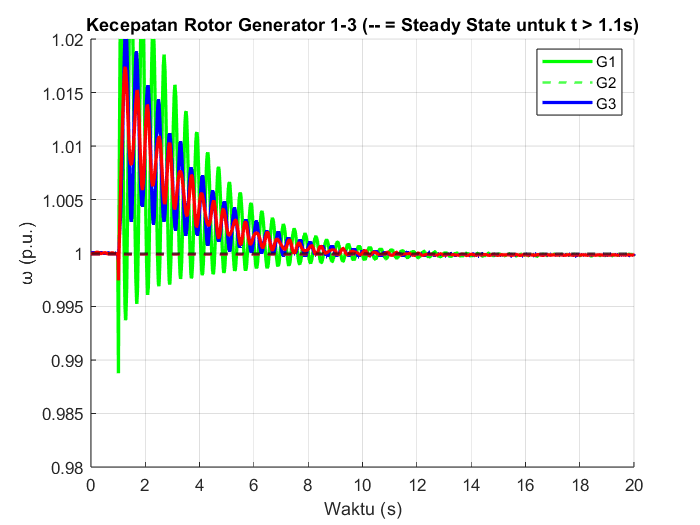
\includegraphics[width=\linewidth]{contents/chapter-4/rocof-pv-fault1.png}
        \caption{Skenario 2}
        \label{Fig:rocof-pv2-fault1}
    \end{subfigure}
    \hfill
    \begin{subfigure}[b]{0.49\linewidth}
        \centering
        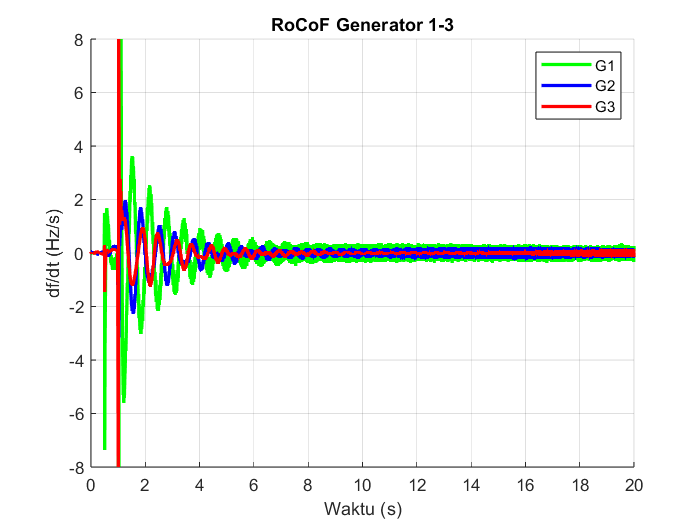
\includegraphics[width=\linewidth]{contents/chapter-4/rocof-vi-fault1.png}
        \caption{Skenario 3}
        \label{Fig:rocof-vi-fault1}
    \end{subfigure}
    \caption{Plot RoCoF dari Gambar \ref{Fig:frek23-fault1}, Gangguan di Bus 1.}
\end{figure}

Pada \ref{Fig:rocof-pv2-fault1} terlihat ... sementara pada \ref{Fig:rocof-vi-fault1} terlihat bahwa ...

\begin{figure}[ht]
    \centering
    \begin{subfigure}[b]{0.49\linewidth}
        \centering
        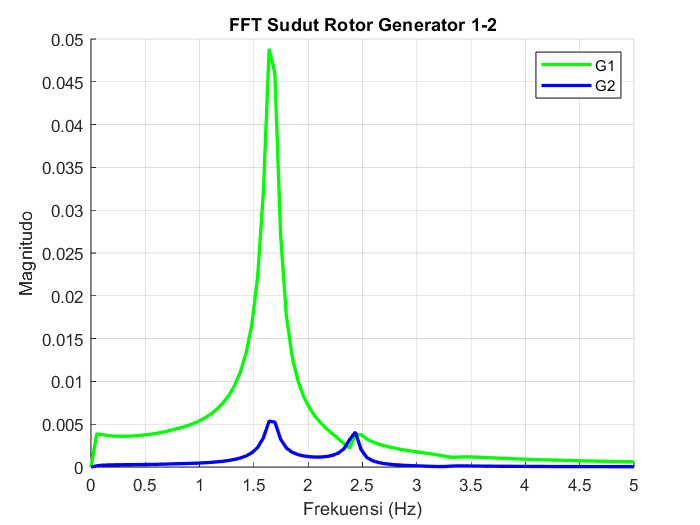
\includegraphics[width=\linewidth]{contents/chapter-4/fft-pv-fault1.png}
        \caption{Skenario 2}
        \label{Fig:fft-pv2-fault1}
    \end{subfigure}
    \hfill
    \begin{subfigure}[b]{0.49\linewidth}
        \centering
        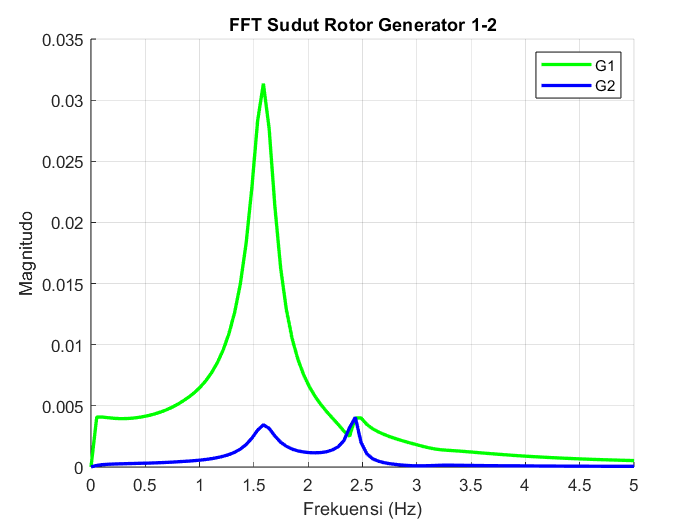
\includegraphics[width=\linewidth]{contents/chapter-4/fft-vi-fault1.png}
        \caption{Skenario 3}
        \label{Fig:fft-vi-fault1}
    \end{subfigure}
    \caption{Plot FFT Kecepatan Rotor dari Gambar \ref{Fig:frek23-fault1}, Gangguan di Bus 1.}
\end{figure}

Pada \ref{Fig:fft-pv2-fault1} terlihat ... sementara pada \ref{Fig:fft-vi-fault1} terlihat bahwa ...



\subsection{Dampak ke Sudut Rotor}

\begin{figure}[ht]
    \centering
    \begin{subfigure}[b]{0.49\linewidth}
        \centering
        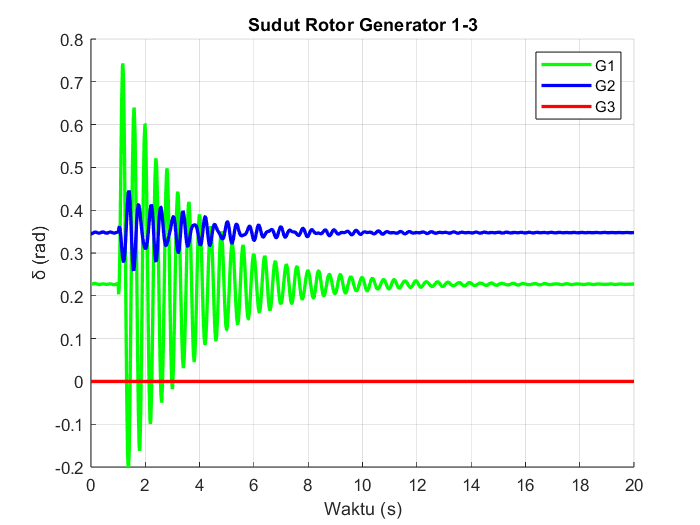
\includegraphics[width=\linewidth]{contents/chapter-4/ang-pv-fault1.png}
        \caption{Skenario 2}
        \label{Fig:ang-pv2-fault1}
    \end{subfigure}
    \hfill
    \begin{subfigure}[b]{0.49\linewidth}
        \centering
        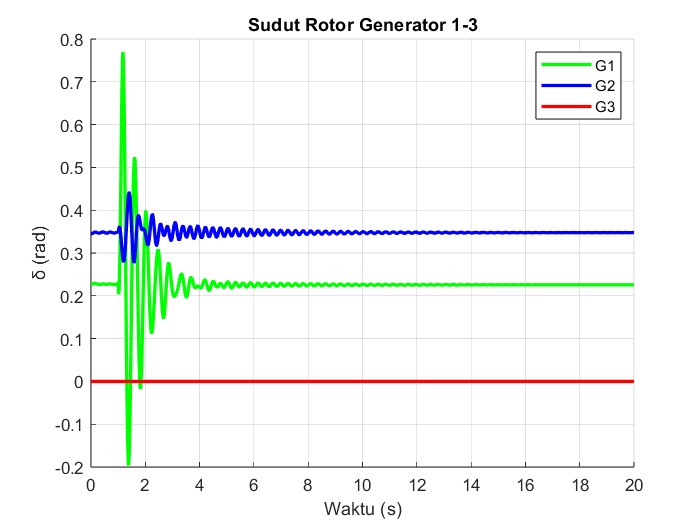
\includegraphics[width=\linewidth]{contents/chapter-4/ang-vi-fault1.png}
        \caption{Skenario 3}
        \label{Fig:ang-vi-fault1}
    \end{subfigure}
    \caption{Plot Sudut Rotor, Gangguan di Bus 1}
    \label{Fig:ang23-fault1}
\end{figure}

Pada \ref{Fig:ang-pv2-fault1} terlihat ... sementara pada \ref{Fig:ang-vi-fault1} terlihat bahwa ...



\section{Temuan Utama}



\subsection{Efek Dinamika Integrasi SPV}



\subsection{Kontribusi Inti dari \textit{Virtual Inertia}}



\subsection{Keterbatasan \textit{Virtual Inertia}}



\subsection{Dampak dari lokasi Gangguan}




\section{Perbandingan dengan Hasil Penelitian Sebelumnya}